\documentclass[11pt,a4paper]{article}

\usepackage[utf8]{inputenc}
\usepackage[T1]{fontenc}
\usepackage[brazil]{babel}
\usepackage{lmodern}
\usepackage{microtype}
\usepackage{amsmath}
\usepackage[a4paper,margin=2cm]{geometry}
\usepackage{graphicx}
\usepackage{subcaption}
\usepackage{booktabs}
\usepackage{tabularx}
\usepackage{array}
\usepackage{xcolor}
\usepackage{enumitem}
\usepackage{caption}
\usepackage{float}
\usepackage[hidelinks]{hyperref}

\captionsetup{font=small,labelfont=bf}
\setlist{nosep,leftmargin=*}
\setlength{\parskip}{0.4em}
\setlength{\parindent}{0pt}
\renewcommand{\arraystretch}{1.15}

% trechos de código e nomes de campos (verde, como no .docx)
\definecolor{codverde}{HTML}{188038}
\newcommand{\cod}[1]{\textcolor{codverde}{\texttt{\small #1}}}
\newcolumntype{L}{>{\raggedright\arraybackslash}X}

\title{\vspace{-1.2cm}Relatório --- Entrega 2: Janela Deslizante (GBN e SR)}
\author{%
  CIC0236 -- Teleinformática e Redes 2 -- Turma 01 -- 2026/2 -- Universidade de Brasília\\[0.4em]
  \textbf{Grupo 10} (\cod{--group grupo10})\\
  Anna Luiza Novaes Jansen Silva -- 232024572\\
  Vinicius Henrique Barbosa Silverio de Castro -- 232006832}
\date{}

\begin{document}
\maketitle
\vspace{-0.5cm}

Todos os testes usam o arquivo \cod{small} (1\,MB, 2\,048 segmentos de 512\,B), timeout fixo de 500\,ms e \cod{--seed 42} (outras seeds só na verificação de robustez, ao fim da Seção~6).

%% ---------------------------------------------------------------------------
\section{Descrição da implementação}

\subsection{Go-Back-N (\cod{gbn.py})}

O GBN mantém uma janela $[\mathit{base}, \mathit{base}+N)$ e \textbf{um único temporizador, o da base}. Não há buffer: só aceita o DATA da base.

\begin{center}\small
\begin{tabularx}{\textwidth}{@{}l l L l@{}}
\toprule
\textbf{Situação} & \textbf{Evento} & \textbf{Ação} & \textbf{Próximo estado}\\
\midrule
Enchendo a janela & \cod{next\_seq < base+N} & envia \cod{REQ(next\_seq)}; se \cod{next\_seq == base}, liga o timer & Enchendo / Esperando\\
Esperando DATA & DATA(\cod{seq == base}) & envia ACK, guarda payload, grava linha do CSV, \cod{base++}, reinicia timer & Enchendo a janela\\
Esperando DATA & DATA(\cod{seq != base}) & descarta (fora de ordem ou duplicata) & Esperando DATA\\
Esperando DATA & timeout da base & marca a base com \cod{timeout\_occurred=1}, reinicia timer, reenvia \cod{REQ(base \ldots\ next\_seq-1)} (``volta N'') & Esperando DATA\\
Esperando DATA & \cod{base == total} & calcula MD5, envia FIN & Encerrando\\
\bottomrule
\end{tabularx}
\end{center}

\textbf{Critério de retransmissão:} estouro do timer da base; reenvia a base e todos os seguintes, mesmo os que já tinham chegado (e foram descartados por estarem fora de ordem). No CSV, \cod{timeout\_occurred=1} marca só o segmento que estava na base (uma vez, ainda que a mesma base estoure mais de uma vez); os reenviados ``de carona'' aparecem apenas em \cod{retransmissions}.

\subsection{Selective Repeat (\cod{sr.py})}

O SR mantém a janela $[\mathit{base}, \mathit{base}+N)$ e \textbf{um temporizador por segmento} (\cod{last\_send[seq] + timeout}). Como há um único socket, \cod{recv\_data} espera até o menor prazo entre os pendentes.

\begin{center}\small
\begin{tabularx}{\textwidth}{@{}l l L l@{}}
\toprule
\textbf{Situação} & \textbf{Evento} & \textbf{Ação} & \textbf{Próximo estado}\\
\midrule
Enchendo a janela & \cod{next\_seq < base+N} & envia \cod{REQ(next\_seq)} e registra \cod{last\_send} & Esperando DATA\\
Esperando DATA & DATA(\cod{seq}) novo na janela & envia \cod{ACK(seq)} individual, guarda em \cod{payloads[seq]} (mesmo fora de ordem), grava linha do CSV & Avançando janela\\
Esperando DATA & DATA duplicado ou fora da janela & descarta & Esperando DATA\\
Esperando DATA & timeout de pendentes & reenvia \cod{REQ} \textbf{só} dos segmentos cujo timer estourou & Esperando DATA\\
Avançando janela & \cod{received[base]} & \cod{base++} (enquanto houver consecutivos recebidos) & Enchendo a janela\\
\bottomrule
\end{tabularx}
\end{center}

\textbf{Segmentos fora de ordem:} ficam em \cod{payloads[seq]} e \cod{received[seq]}; o arquivo é remontado na ordem do \cod{seq}, o que o MD5 confirma (Seção~\ref{sec:md5}).

\begin{figure}[ht]
  \centering
  \begin{subfigure}[t]{0.49\textwidth}
    \centering
    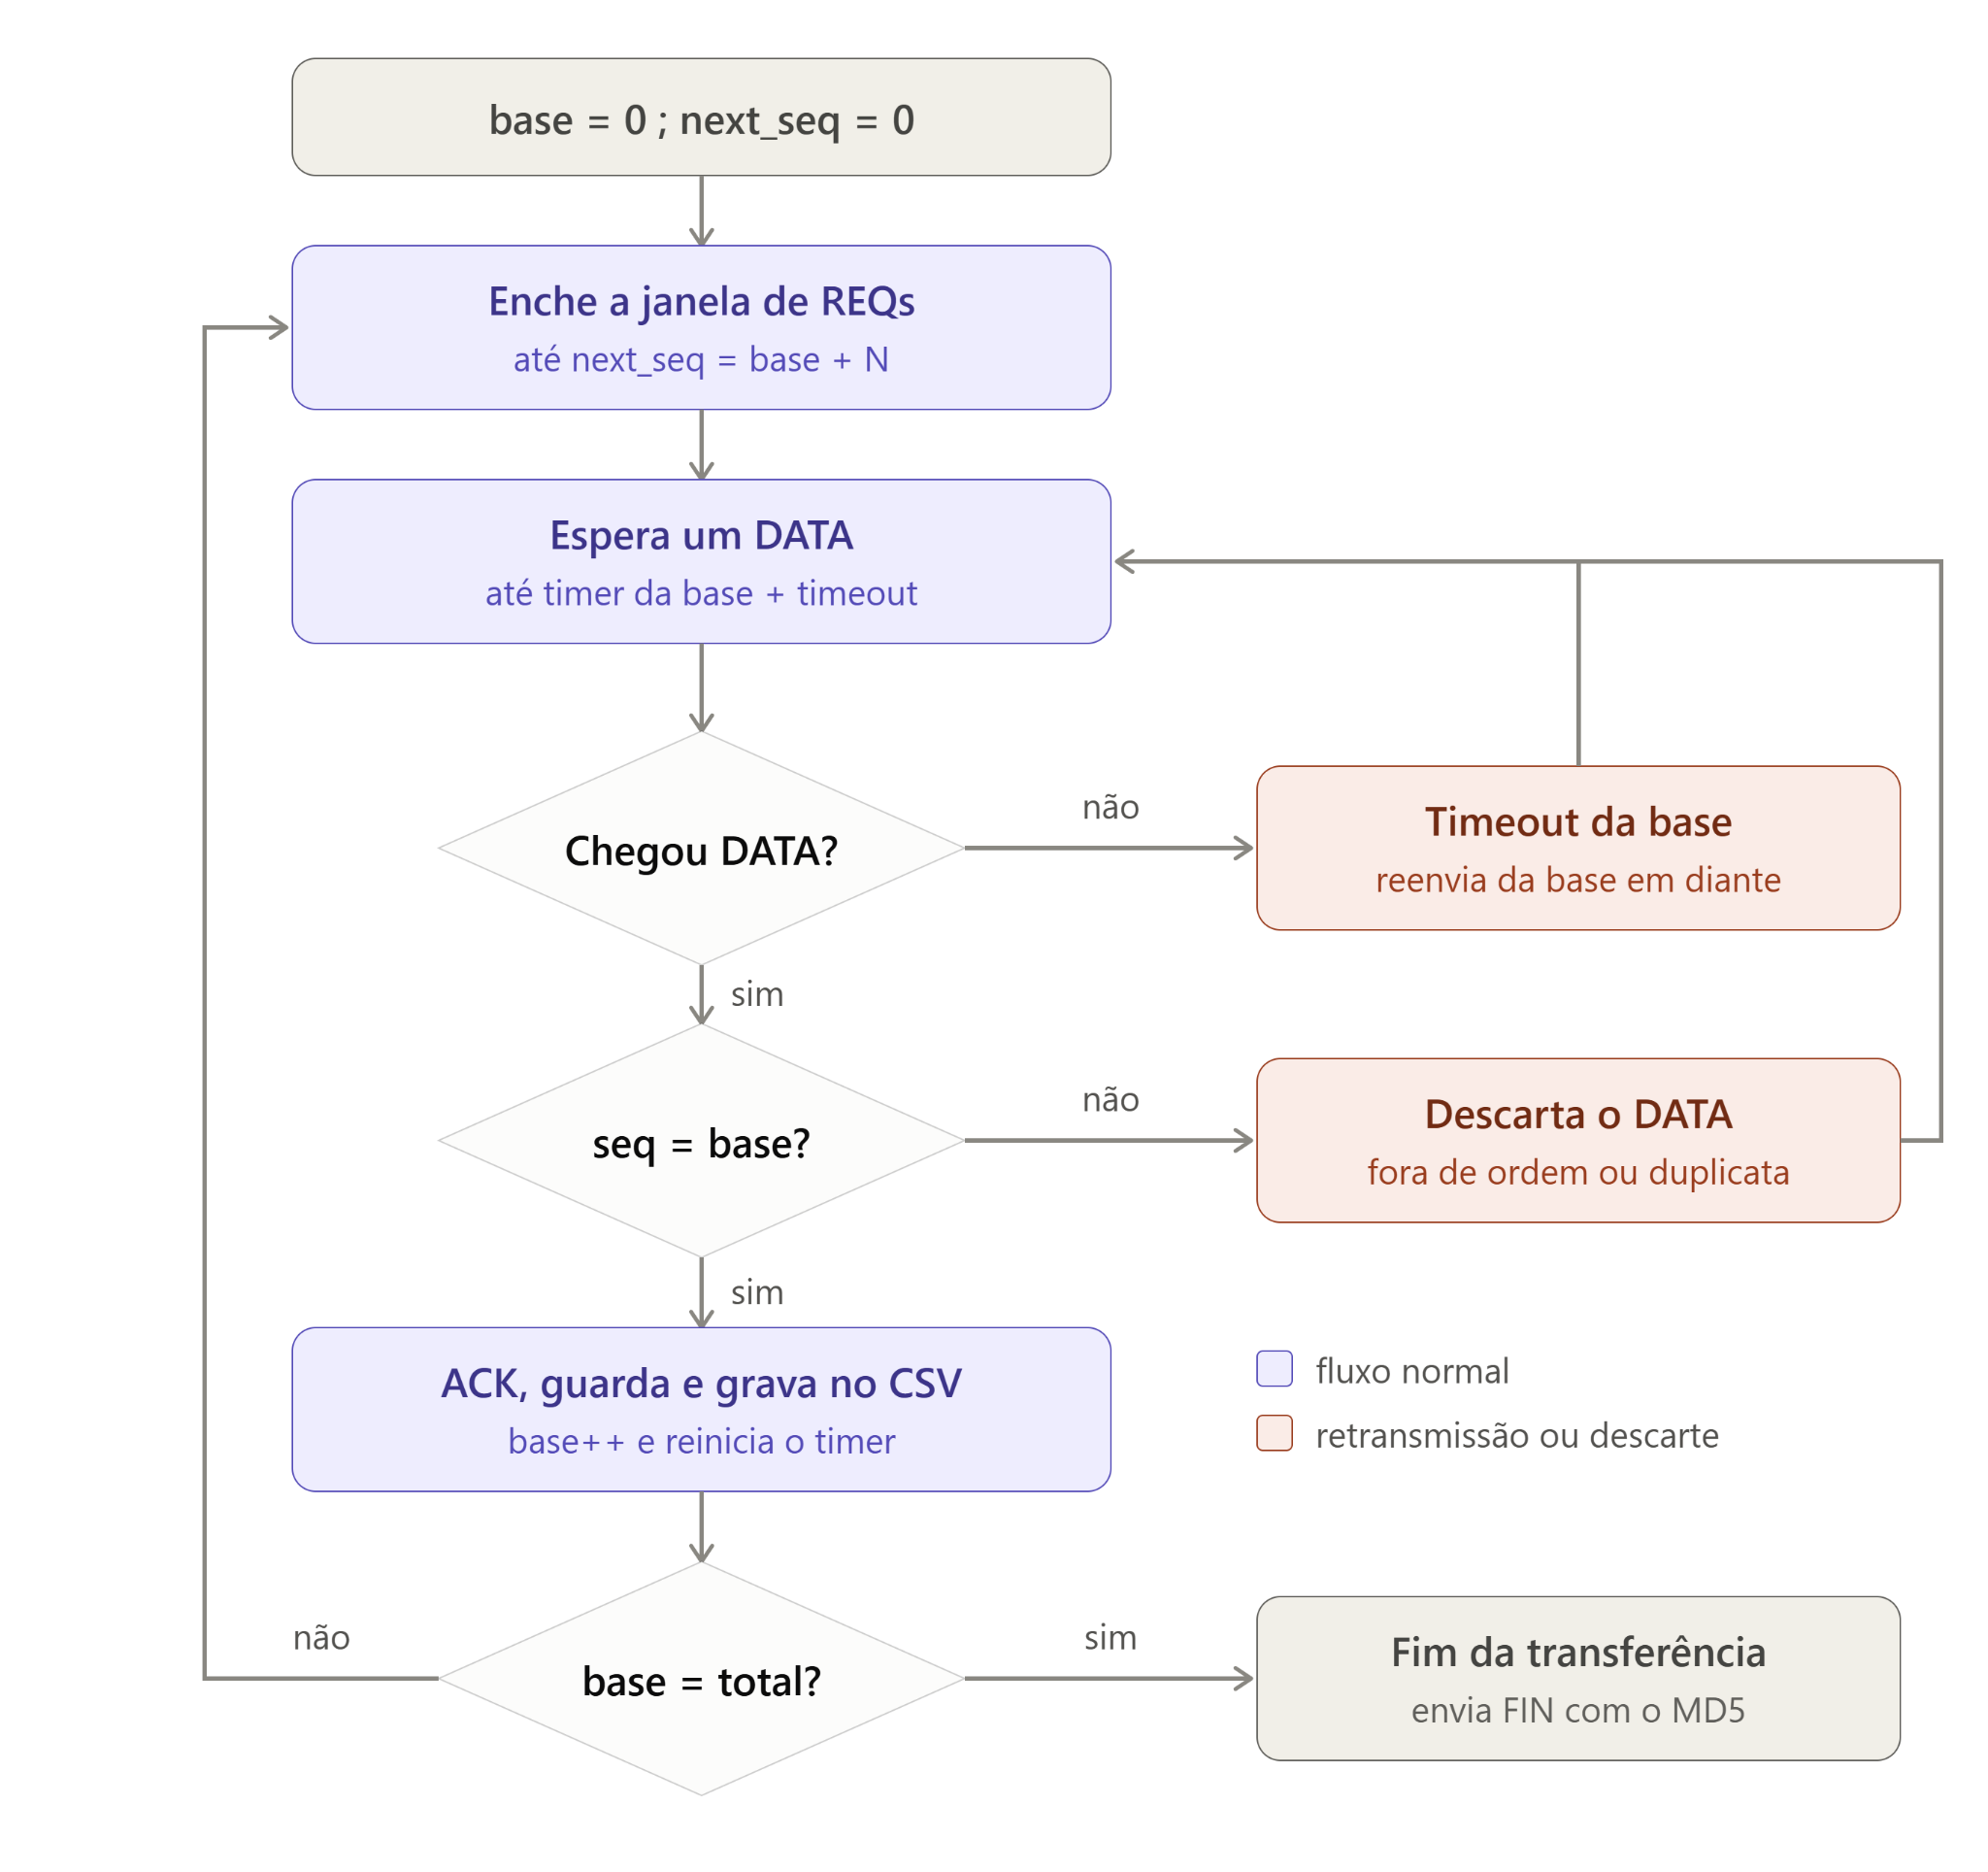
\includegraphics[width=\linewidth]{figuras/fluxograma_gbn.png}
    \caption{Go-Back-N}
  \end{subfigure}\hfill
  \begin{subfigure}[t]{0.49\textwidth}
    \centering
    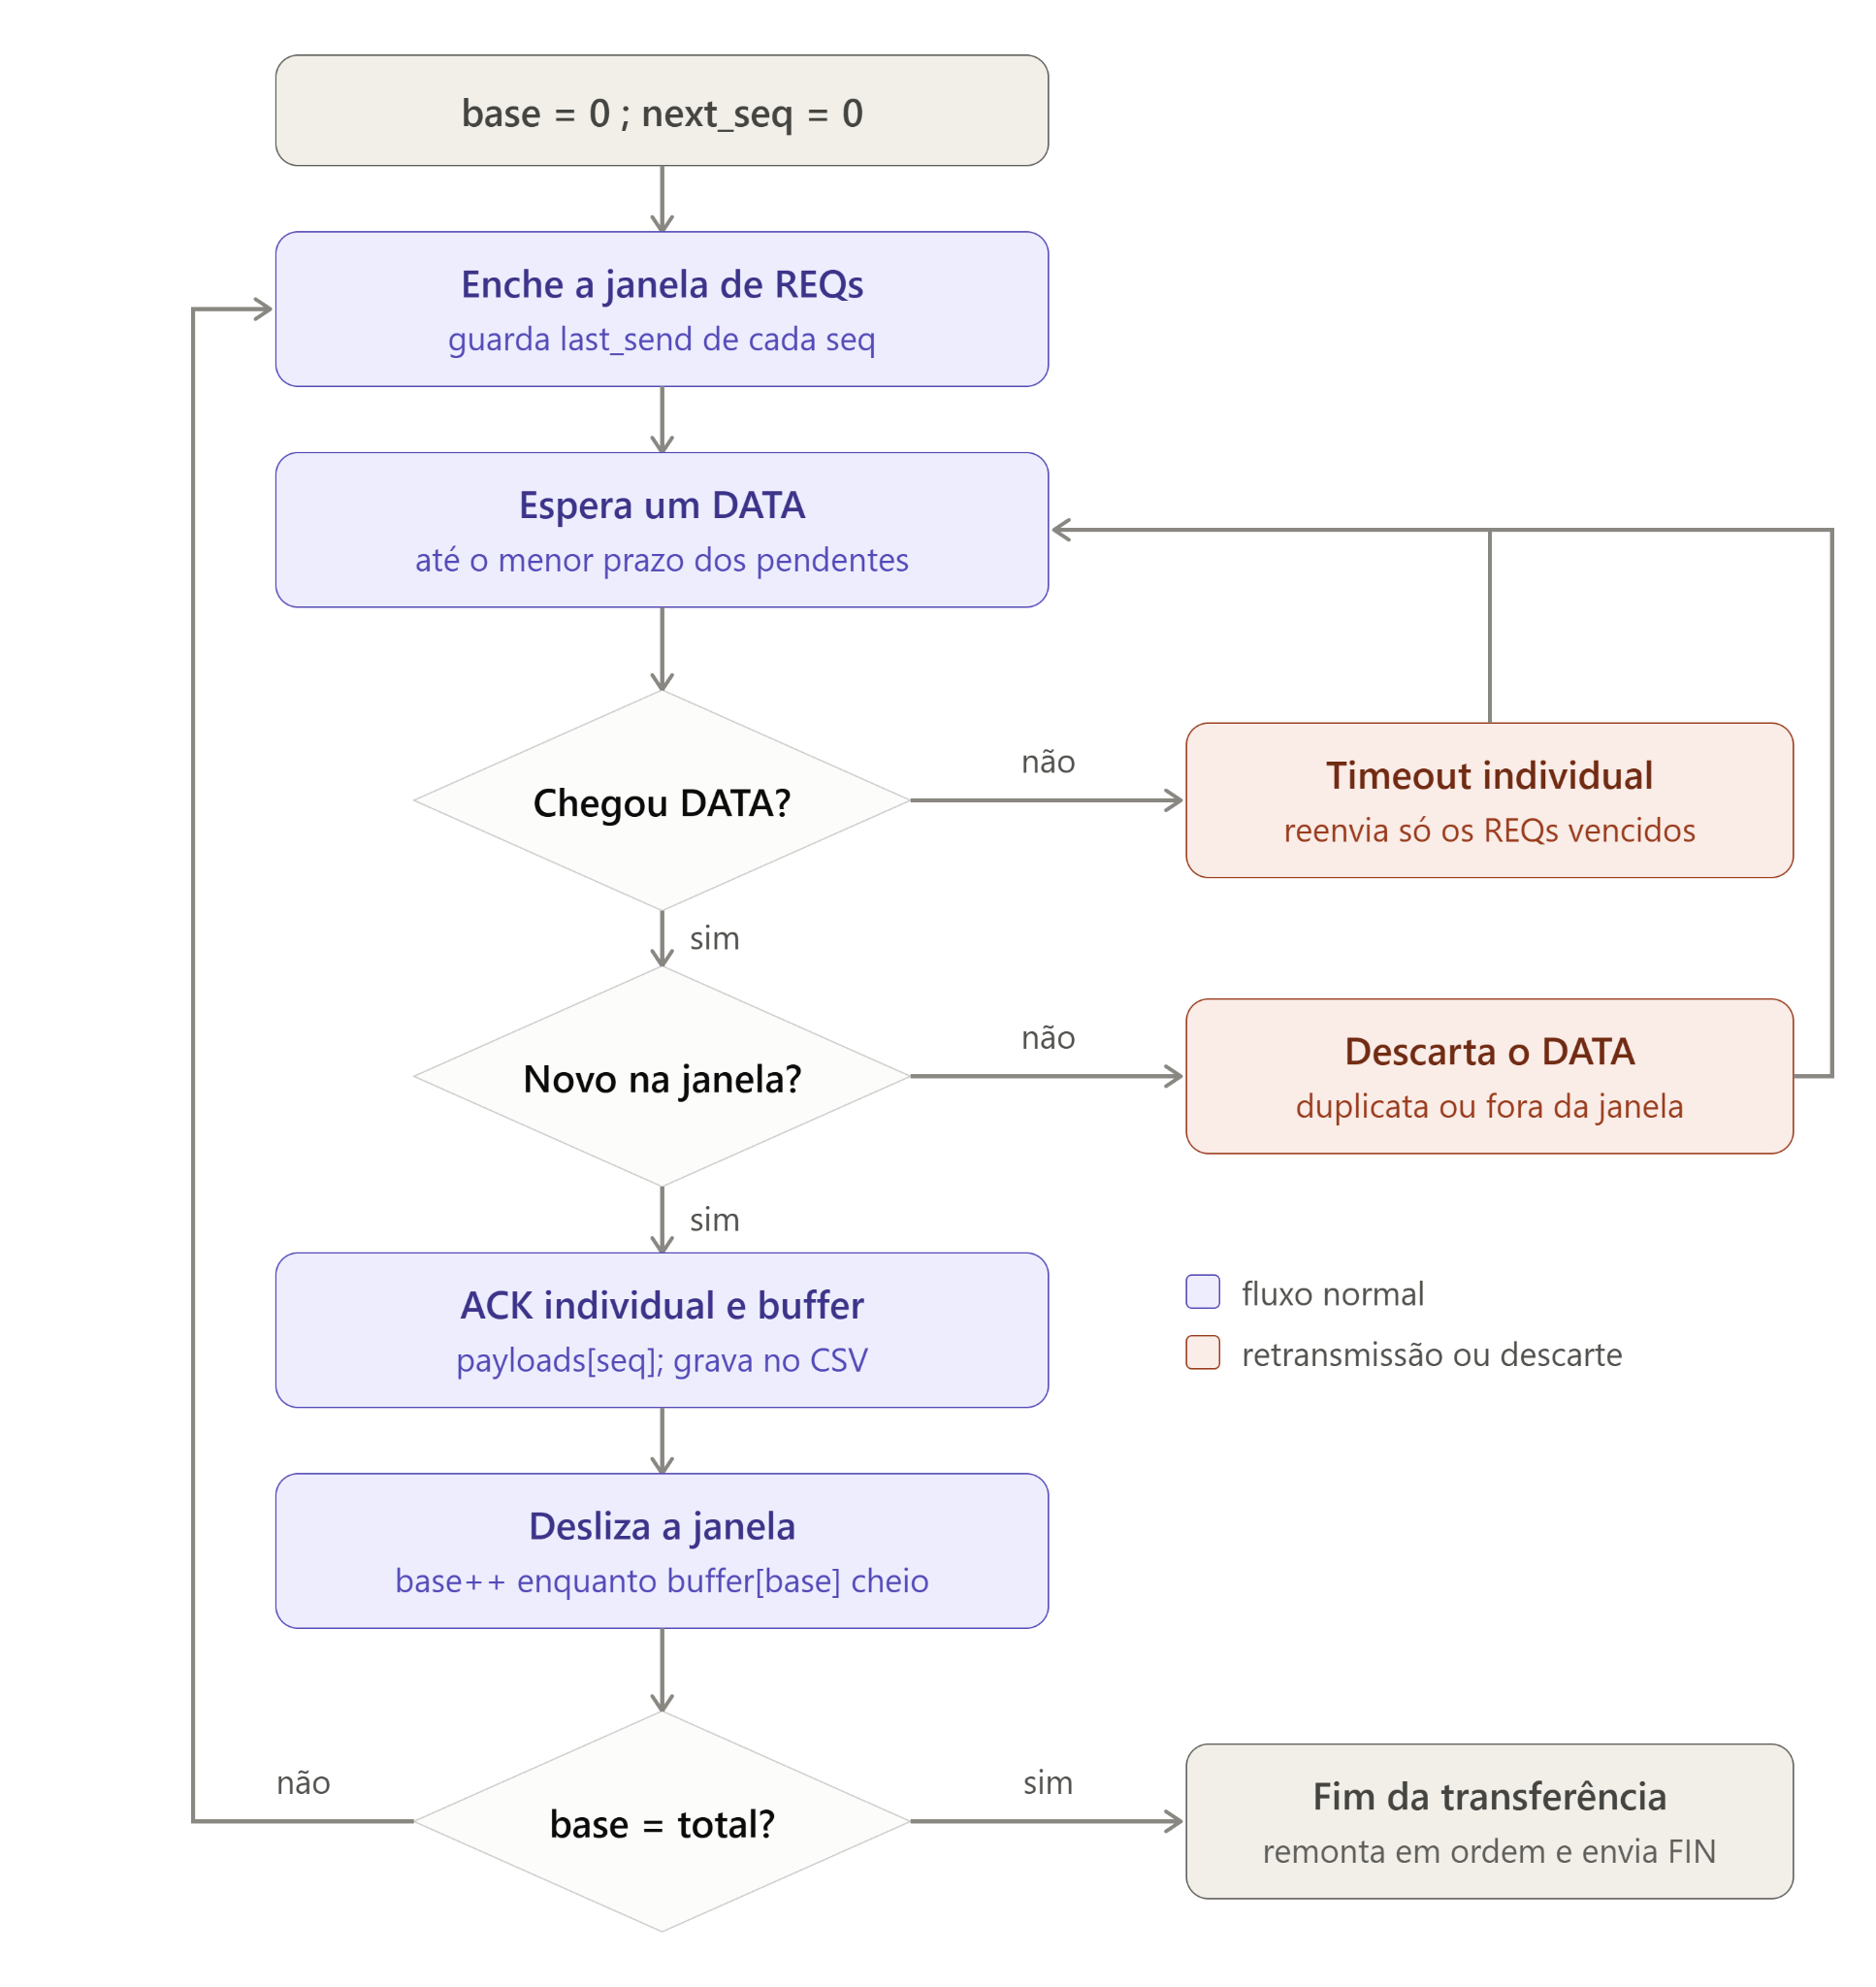
\includegraphics[width=\linewidth]{figuras/fluxograma_sr.png}
    \caption{Selective Repeat}
  \end{subfigure}
  \caption{Fluxogramas do cliente. Em vermelho, os caminhos de retransmissão e descarte: no GBN o timeout é só o da base e reenvia a janela inteira; no SR cada segmento tem seu timer e só os vencidos são reenviados.}
  \label{fig:fluxogramas}
\end{figure}

%% ---------------------------------------------------------------------------
\section{Método de simulação de perda}

\textbf{Abordagem escolhida: (a), descartar o DATA recebido com probabilidade $P$} (\cod{--loss}). O DATA chega de verdade, mas, dentro de \cod{comum.recv\_data}, é descartado antes de qualquer processamento, como se a rede o tivesse perdido. O efeito no protocolo é o de uma perda real: o temporizador estoura e o REQ é reenviado.

\textbf{Por que não a (b)} (receber o DATA e não enviar o ACK): o servidor é \emph{pull-based} e o cliente só avança ao receber o DATA. Deixar de enviar o ACK não provoca timeout nem retransmissão, então a (b) não simularia perda nenhuma neste protocolo.

\textbf{Ponto único de aplicação:} SAW, GBN e SR recebem DATA pelo mesmo \cod{recv\_data}, então a perda é aplicada de forma idêntica nos três. HELLO/OK e FIN/DONE não passam pela simulação.

\textbf{Repetibilidade:} o sorteio usa \cod{random.Random(seed)}; todos os cenários oficiais usam \cod{--seed 42}, registrada no \cod{resumo\_entrega2.csv}. Sem \cod{--loss}, nenhum sorteio é feito.

\textbf{Registro no CSV} (colunas acrescentadas às da especificação):

\begin{center}\small
\begin{tabular}{@{}l l@{}}
\toprule
\textbf{Coluna} & \textbf{Significado}\\
\midrule
\cod{simulated\_loss} & 1 se algum DATA deste segmento foi descartado pela simulação\\
\cod{sim\_drops} & quantos DATA deste segmento foram descartados\\
\cod{recv\_time\_ms} & instante da aceitação desde o início da transferência\\
\bottomrule
\end{tabular}
\end{center}

No SAW e no SR, uma retransmissão em segmento com \cod{simulated\_loss = 0} seria perda natural da rede UDP. Nos 21 cenários oficiais ela foi \textbf{zero}: em todos os cenários do SAW e do SR, o total de retransmissões é igual ao de DATA descartados pela simulação (91 com 5\,\%, 220 com 10\,\%), e os cenários sem perda simulada não tiveram nenhuma retransmissão. No GBN essa separação é diferente: os segmentos reenviados ``de carona'' no ``volta N'' também têm \cod{simulated\_loss = 0} (1\,202 segmentos no GBN-16 com 10\,\%), sem que tenha havido perda natural.

\textbf{Observação:} o sorteio é feito \textbf{por DATA recebido}, não por segmento. No GBN cada segmento chega várias vezes (por causa do ``volta N''), então ele consome mais sorteios e tem mais descartes que SAW e SR com a mesma seed (541 contra 220 com 10\,\%). A probabilidade por pacote é a mesma para todos.

%% ---------------------------------------------------------------------------
\section{Checksum MD5}\label{sec:md5}

Todos os 21 cenários (SAW, GBN e SR $\times$ janelas 4/8/16 $\times$ 0\,\%, 5\,\% e 10\,\%) terminaram com o mesmo MD5, igual ao informado pelo servidor no OK, e com \cod{DONE ok=1}:
\begin{center}
\cod{f989450f6ca695013ceb6bd3a5f6417c}
\end{center}
O MD5 é o mesmo em todos porque o arquivo \cod{small} do grupo 10 é sempre o mesmo. Isso confirma que a reordenação do SR e a remontagem do GBN estão corretas, mesmo com 10\,\% de perda.

%% ---------------------------------------------------------------------------
\section{Tabela comparativa}

Cada célula traz \textbf{throughput médio (kbps) / total de retransmissões / tempo total (s)}, com throughput $= \text{file\_size} \times 8 / \text{tempo\_total}$. Cada cenário foi executado uma vez com \cod{--seed 42}.

\begin{table}[ht]
\centering\small
\begin{tabular}{@{}l c r r r@{}}
\toprule
\textbf{Protocolo} & \textbf{Janela} & \textbf{Sem perda} & \textbf{5\,\% de perda} & \textbf{10\,\% de perda}\\
\midrule
SAW & 1  & 167,2 / 0 / 50,2   & 88,3 / 91 / 95,0    & 52,0 / 220 / 161,3\\
\midrule
GBN & 4  & 657,7 / 0 / 12,8   & 140,7 / 360 / 59,6  & 63,8 / 921 / 131,5\\
GBN & 8  & 1235,5 / 0 / 6,8   & 152,0 / 744 / 55,2  & 66,9 / 1848 / 125,4\\
GBN & 16 & 2025,5 / 0 / 4,1   & 159,5 / 1512 / 52,6 & 70,3 / 3562 / 119,3\\
\midrule
SR  & 4  & 635,2 / 0 / 13,2   & 161,6 / 91 / 51,9   & 84,4 / 220 / 99,5\\
SR  & 8  & 1162,5 / 0 / 7,2   & 192,7 / 91 / 43,5   & 109,6 / 220 / 76,5\\
SR  & 16 & 1900,7 / 0 / 4,4   & 260,7 / 91 / 32,2   & 153,7 / 220 / 54,6\\
\bottomrule
\end{tabular}
\caption{Comparação SAW $\times$ GBN $\times$ SR: throughput médio (kbps) / retransmissões / tempo total (s).}
\label{tab:comparativa}
\end{table}

\textbf{Nota:} o SAW sem perda atingiu 167\,kbps aqui contra $\sim$64\,kbps na Entrega~1 (\cod{small}). A diferença se deve às condições da rede em cada dia (RTT médio de $\sim$24\,ms agora contra $\sim$38\,ms antes, com perda natural diferente).

%% ---------------------------------------------------------------------------
\section{Gráficos por segmento}

\begin{figure}[H]
  \centering
  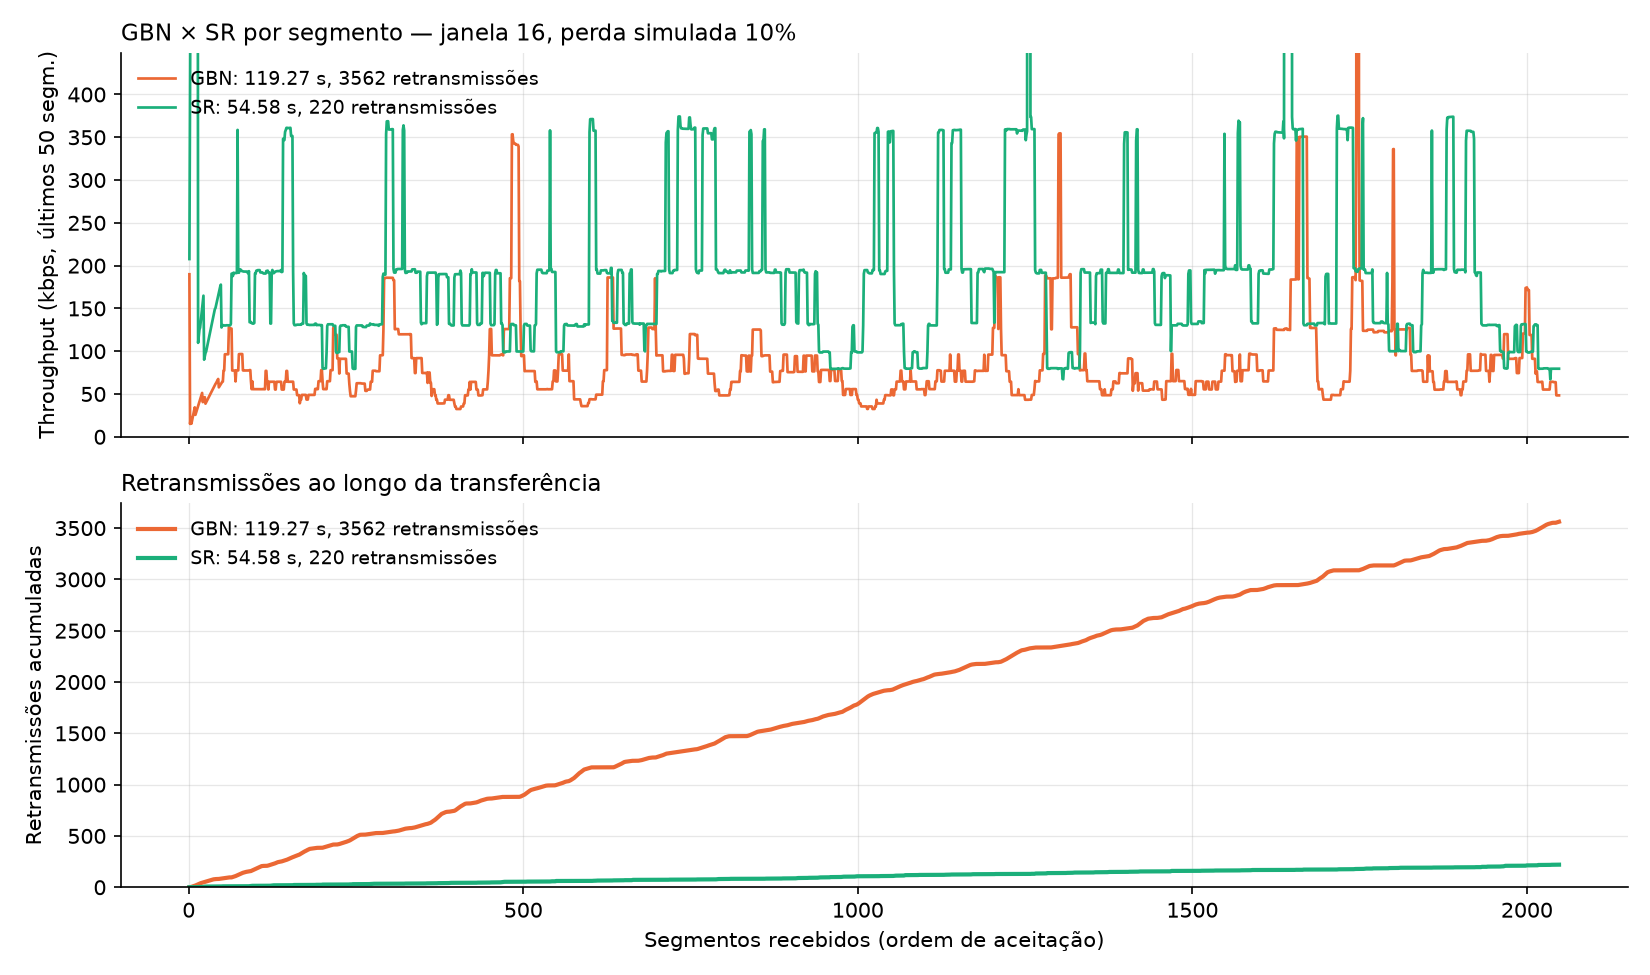
\includegraphics[width=0.92\textwidth]{figuras/comparacao_segmentos_w16_loss10.png}
  \caption{GBN $\times$ SR, janela 16, 10\,\% de perda: throughput (média dos últimos 50 segmentos) e retransmissões acumuladas ao longo da transferência. O GBN acumula retransmissões em saltos de até 16 a cada timeout; no SR a curva sobe de 1 em 1.}
  \label{fig:seg10}
\end{figure}

\begin{figure}[H]
  \centering
  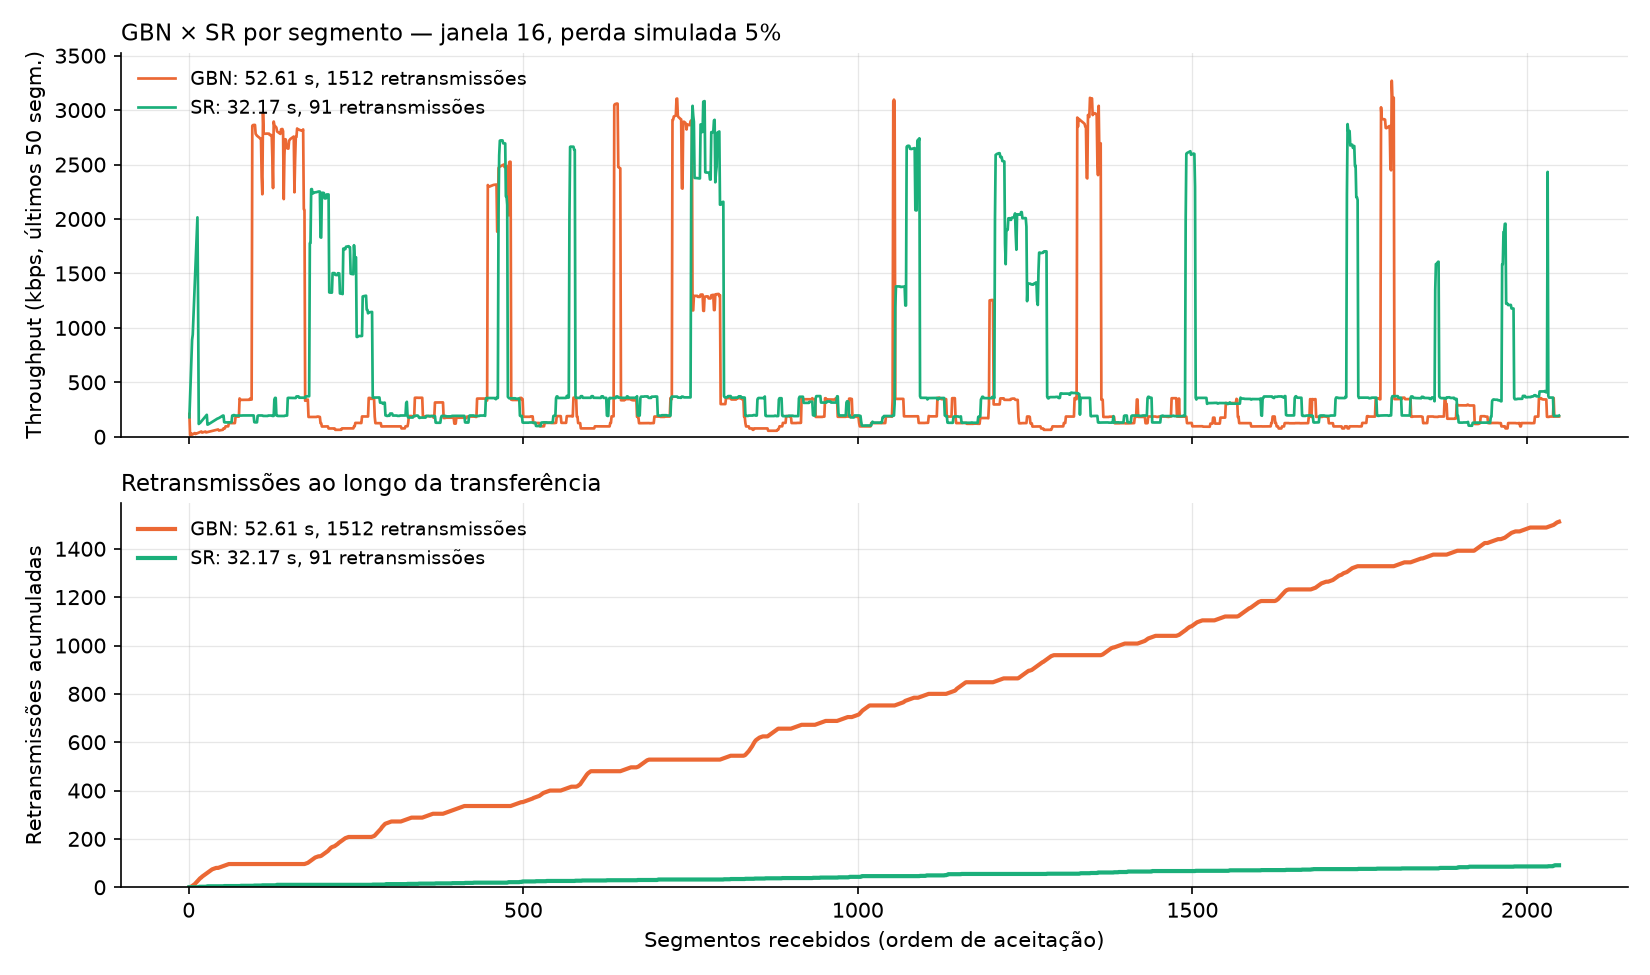
\includegraphics[width=0.92\textwidth]{figuras/comparacao_segmentos_w16_loss5.png}
  \caption{Mesma comparação com 5\,\% de perda.}
  \label{fig:seg5}
\end{figure}

%% ---------------------------------------------------------------------------
\section{Análise}

\subsection*{a) Impacto da janela no throughput sem perda}

Sem perda, a janela multiplica a vazão, pois $\text{throughput} \approx N \times L / \text{RTT}$: SAW 167\,kbps $\to$ $N=4$ $\sim$650 $\to$ $N=8$ $\sim$1\,200 $\to$ $N=16$ $\sim$2\,000\,kbps, com eficiência de $\sim$99\,\% em todos os casos (medido $\div$ teórico). O ganho com $N=16$ é de $\sim$12$\times$ e não 16$\times$, porque o RTT médio sobe de $\sim$24\,ms para $\sim$32--34\,ms com 16 REQs em voo (enfileiramento). Sem perda, GBN e SR se comportam de forma praticamente igual ($N=8$: 1\,236 contra 1\,163\,kbps), pois a diferença entre eles só aparece quando há retransmissão.

\textbf{Estabilização:} nas janelas obrigatórias (4, 8 e 16) o throughput ainda cresce a cada dobra, com retorno decrescente (4$\to$8: 1,88$\times$; 8$\to$16: 1,64$\times$). Para achar o ponto de estabilização, rodamos uma varredura extra sem perda em 28/10 (GBN e SR, $N = 4, 8, 16, 24, 32, 48, 64, 96, 128$, duas rodadas cada, todas com MD5 correto; \cod{resultados/janela\_estabilizacao/}). A Figura~\ref{fig:estab} mostra o resultado: o throughput cresce quase linearmente até $N=16$ ($\sim$2\,000\,kbps), desacelera em $N=24$--32 ($\sim$2\,300--2\,500\,kbps) e \textbf{estabiliza a partir de $N \approx 32$--48, em $\sim$2\,700--2\,900\,kbps} (SR: 2\,742 / 2\,774 / 2\,901 / 2\,782\,kbps em $N=48/64/96/128$). Dobrar a janela de 48 para 96 rende só $\sim$6\,\%.

\textbf{Por quê:} enquanto $N \times L$ é menor que o produto banda $\times$ atraso, o cliente fica ocioso esperando DATA, e cada REQ a mais em voo vira vazão a mais, com o RTT praticamente constante ($\sim$30--33\,ms até $N=16$). Com um RTT base de $\sim$30\,ms e um gargalo de $\sim$2,8\,Mbps, esse produto é $2{,}8\,\text{Mbps} \times 30\,\text{ms} \approx 84\,\text{kbit} \approx 20$ segmentos de 512\,B: é exatamente onde a curva dobra. Acima disso o caminho (rede ou taxa de atendimento do servidor) já está sempre ocupado, e os REQs extras só esperam em fila: o RTT passa a crescer \textbf{proporcionalmente a $N$} (39\,ms em $N=24$, 50\,ms em 32, 71\,ms em 48, 93\,ms em 64, $\sim$130\,ms em 96), de modo que $N/\text{RTT}$ fica constante em $\sim$700 segmentos/s ($\approx 1{,}4$\,ms por segmento). Ou seja, aumentar a janela além de $\sim$32 não aumenta a vazão, só a fila.

Janelas grandes demais chegam a piorar: em $N=128$ a fila transborda e aparecem perdas naturais (sem \cod{--loss}). O SR retransmite só os perdidos (64--73 retransmissões) e mantém $\sim$2\,780\,kbps, mas o GBN reenvia a janela inteira a cada timeout (604--724 retransmissões) e cai para $\sim$1\,700\,kbps. Perdas naturais esporádicas (1--2 timeouts) aparecem também em janelas menores, mas custam muito mais ao GBN (até 107 retransmissões em $N=96$) que ao SR (no máximo 6). Para este servidor, uma janela em torno de \textbf{32--48} dá o throughput máximo sem encher a fila à toa.

\begin{figure}[H]
  \centering
  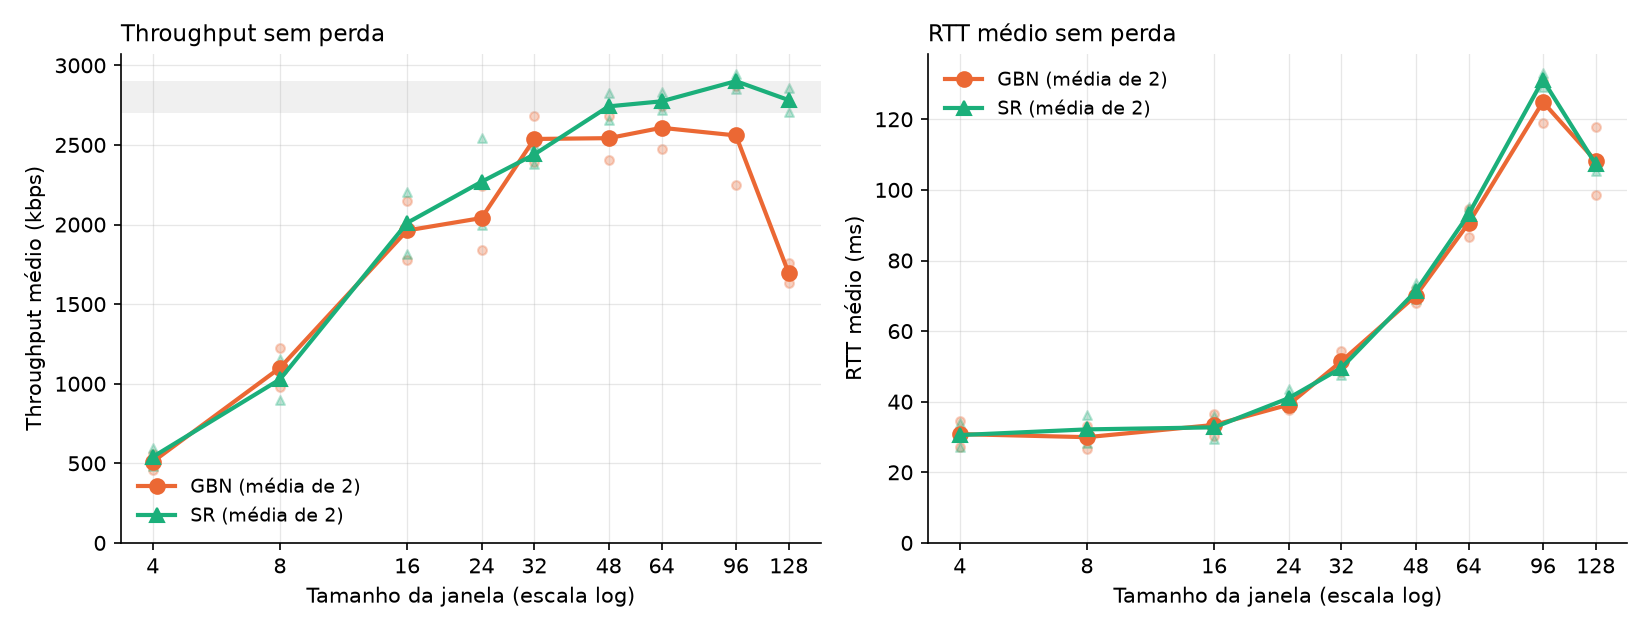
\includegraphics[width=0.92\textwidth]{figuras/estabilizacao_janela.png}
  \caption{Varredura extra sem perda (28/10): throughput (esquerda) e RTT médio (direita) conforme a janela, em escala log. Pontos claros: cada rodada; linha: média das duas. A faixa cinza marca o patamar de $\sim$2\,700--2\,900\,kbps. A partir de $N \approx 32$ o throughput para de crescer e o RTT passa a crescer na proporção de $N$ (fila); em $N=128$ surgem perdas naturais, que derrubam o GBN.}
  \label{fig:estab}
\end{figure}

\begin{figure}[H]
  \centering
  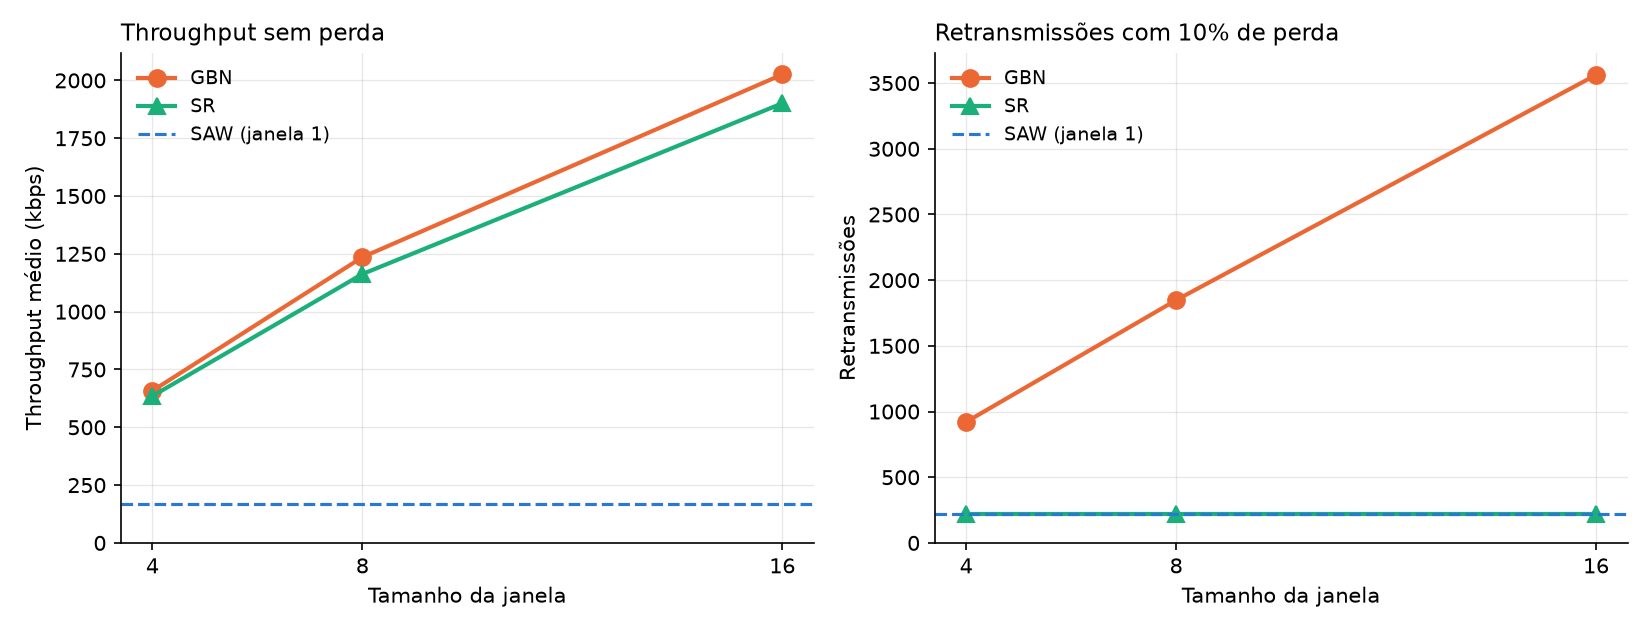
\includegraphics[width=0.92\textwidth]{figuras/comparacao_janela.png}
  \caption{Esquerda: throughput sem perda conforme a janela (item a), com o SAW como referência. Direita: retransmissões com 10\,\% de perda conforme a janela (item b): no GBN crescem com $N$; no SR ficam iguais às do SAW.}
  \label{fig:janela}
\end{figure}

\subsection*{b) Retransmissões por erro (10\,\% de perda, janela 16)}

\begin{center}\small
\begin{tabular}{@{}l r r r r@{}}
\toprule
 & \textbf{Segm.\ com timeout} & \textbf{Timeouts (eventos)$^*$} & \textbf{Retransmissões} & \textbf{Retx.\ $\div$ timeout}\\
\midrule
GBN-16 & 207 & $\geq$ 223 & 3\,562 & $\leq$ 16\\
SR-16  & 191 & 220        & 220    & 1,0\\
\bottomrule
\end{tabular}

\footnotesize $^*$No GBN, estouros do temporizador único da base; no SR, expirações dos temporizadores individuais de cada segmento.
\end{center}

A coluna \cod{timeout\_occurred} do CSV conta \emph{segmentos} que sofreram timeout, não eventos: no GBN, se a mesma base estoura duas vezes, ela é marcada uma vez só. Por isso o número de eventos é obtido das retransmissões. No \textbf{GBN}, cada timeout reenvia a base e os segmentos seguintes já pedidos (no máximo 16), logo houve pelo menos $3\,562 \div 16 \approx 223$ timeouts. No CSV, 1\,667 dos 2\,048 segmentos foram retransmitidos ao menos uma vez (até 7 vezes), e 1\,202 deles nunca tiveram um DATA próprio descartado. No \textbf{SR}, cada timeout reenvia exatamente um segmento: as 220 retransmissões coincidem com os 220 DATA descartados pela simulação (soma de \cod{sim\_drops}), em 191 segmentos (165 reenviados uma vez, 23 duas e 3 três vezes, quando o próprio reenvio também foi descartado). Contando por DATA descartado, o GBN fez $3\,562 \div 541 \approx 6{,}6$ retransmissões por descarte. Em números absolutos, o GBN-16 retransmitiu \textbf{16$\times$ mais} que o SR-16 nas mesmas condições de perda.

\subsection*{c) Por que o GBN sofre mais que o SR com perda alta}

\begin{figure}[H]
  \centering
  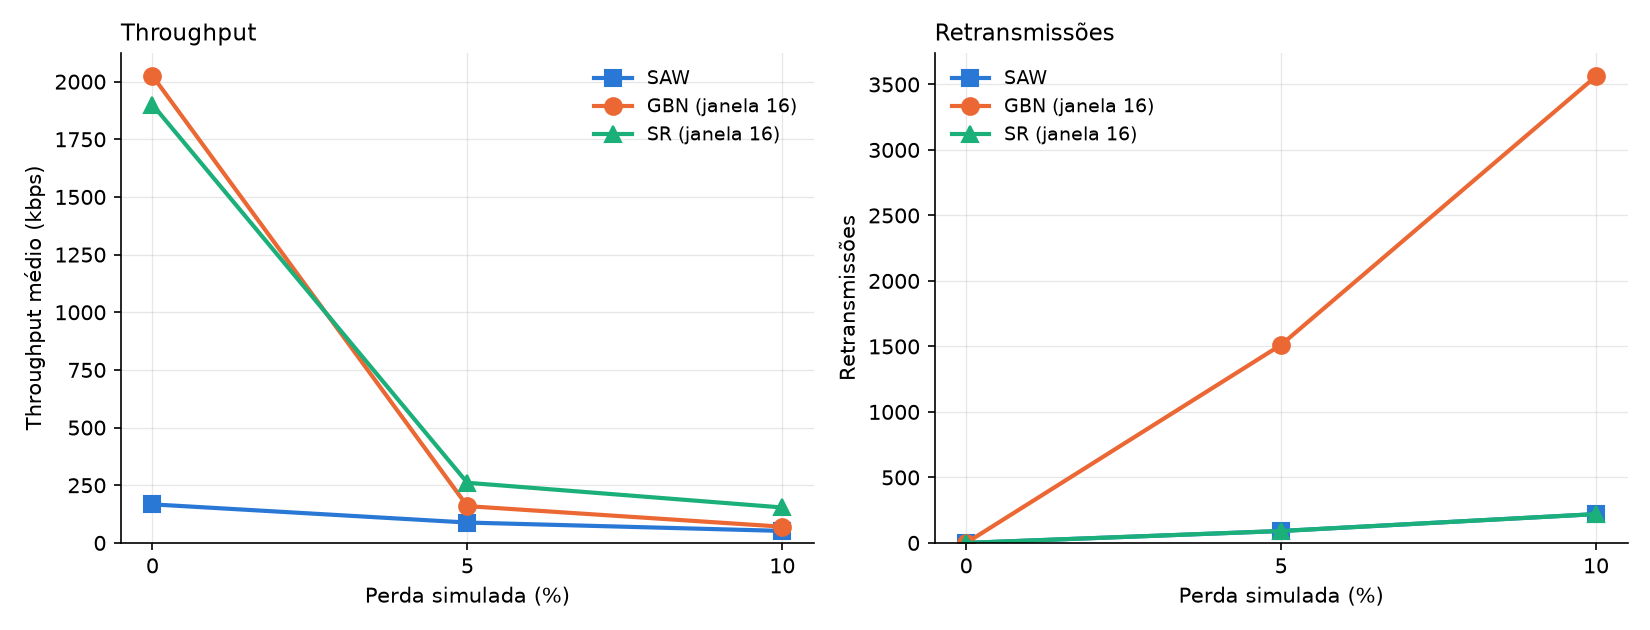
\includegraphics[width=0.92\textwidth]{figuras/comparacao_perda.png}
  \caption{SAW, GBN-16 e SR-16 conforme a perda simulada: throughput médio (esquerda) e retransmissões (direita).}
  \label{fig:perda}
\end{figure}

\begin{enumerate}[label=\arabic*.]
  \item \textbf{Volume de retransmissões.} Com 10\,\% de perda, o GBN-16 retransmite 3\,562 segmentos contra 220 do SR; com 5\,\%, 1\,512 contra 91 ($\sim$16,6$\times$). O GBN reenvia a janela inteira a cada timeout, e cada reenvio extra é também um DATA exposto a novas perdas.
  \item \textbf{Os timeouts do GBN se somam; os do SR se sobrepõem.} No GBN cada timeout trava todo o progresso: pelo menos $223 \times 0{,}5\,\text{s} \approx 112$\,s dos 119,3\,s do GBN-16 foram gastos esperando timeouts. No SR, enquanto um segmento espera o timeout, os outros da janela continuam chegando e vão para o buffer: os 220 timeouts do SR-16 somariam 110\,s se fossem sequenciais, mas a transferência terminou em \textbf{54,6\,s}. Contando no CSV os intervalos de mais de 300\,ms sem nenhuma chegada, o SR-16 teve só 98 paradas para 220 timeouts (vários timers da mesma janela vencem juntos e uma única espera recupera várias perdas), enquanto o GBN-16 teve 207.
  \item \textbf{A janela só ajuda o SR com perda.} Com 10\,\% de perda, o throughput do GBN quase não cresce com $N$ (63,8 $\to$ 66,9 $\to$ 70,3\,kbps), enquanto o do SR cresce bastante (84,4 $\to$ 109,6 $\to$ 153,7\,kbps): quanto maior $N$, mais trabalho útil acontece durante cada espera por timeout. O SR-16 com 10\,\% de perda (153,7\,kbps) chega perto do SAW \emph{sem} perda (167,2\,kbps), enquanto o GBN-16 com 10\,\% (70,3\,kbps) fica abaixo da metade.
\end{enumerate}

\textbf{Robustez à seed:} para verificar que o resultado não depende da sequência sorteada, repetimos GBN-16 e SR-16 com 10\,\% de perda e as seeds 7 e 123 (em \cod{resultados/robustez\_seed/}, todas com MD5 correto):

\begin{center}\small
\begin{tabular}{@{}c r r r r r@{}}
\toprule
\textbf{Seed} & \textbf{Retx.\ GBN-16} & \textbf{Retx.\ SR-16} & \textbf{GBN $\div$ SR} & \textbf{Tempo GBN-16 (s)} & \textbf{Tempo SR-16 (s)}\\
\midrule
42  & 3\,562 & 220 & 16,2$\times$ & 119,3 & 54,6\\
7   & 3\,825 & 231 & 16,6$\times$ & 127,7 & 51,7\\
123 & 3\,634 & 248 & 14,7$\times$ & 121,8 & 54,9\\
\bottomrule
\end{tabular}
\end{center}

Nas três seeds o GBN retransmitiu $\sim$15--17$\times$ mais e levou mais que o dobro do tempo do SR. Na seed 123 o SR teve 248 retransmissões para 247 DATA descartados pela simulação: a única retransmissão sem \cod{simulated\_loss} é uma perda natural da rede, separada justamente por esse campo.

\end{document}
